\chapter{Project Quality Management}

The aim of Quality Management is to manage the quality of the final software product, and the quality of the development process used to create it. Another measure of quality is ensuring that the final product meets the requirements as defined by the stakeholders. 

\section{Quality Process}

The process following for quality would focus on three areas.

\begin{enumerate}
\item Plan Quality Management
\item Perform Quality Assurance
\item Control Quality
\end{enumerate}

\subsection{Quality Management}

Quality Management is the process of "identifying quality requirements and standards for the project" \parencite{pmbok}. It is also important that the project demonstrates "compliance with relevant quality requirements and standards" \parencite{pmbok}. This project focuses on a number of quality attributes during the development process.\newpage

\begin{enumerate}
\item Performance
\begin{itemize}
\item The ability of the project to respond to requests with clearly defined time constraints. For this project, the reaction time the the web application to user demanded is important.
\end{itemize}
\item Security
\begin{itemize}
\item The protection, integrity and non-repudiation of stored data. User information, such as payment information, will be stored. The security of this data is integral to the application.
\end{itemize}
\item Usabilty
\begin{itemize}
\item The system must be easy to use, and easy to learn. Usability studies need to be performed on the application to ensure ease of use.
\end{itemize}
\item Maintainability
\begin{itemize}
\item It must not be cost prohibitive to perform corrective, perfective and adaptive maintenance on the product. The project must be designed in such a way that any changes that need to be made can be done at minimal cost. 
\end{itemize}
\item Re-usability
\begin{itemize}
\item Components of the system must be design modularly in order to promote reuse. A reusable system, if the risk is managed correctly, will save costs if components are reusable, and may also allow further product lines.
\end{itemize}
\item Portability
\begin{itemize}
\item The project application must work across a range of operating systems and browsers.
\end{itemize}
\end{enumerate}

The project aims to conform to the ISO 25010 standard detailed later in this report.

\subsection{Quality Assurance}

Quality Assurance is governed by the user of standards, such as the ISO 25010, within the project. In a big organisation, the idea of Total Quality Management is used to ensure that a high quality product is delivered. This draws on a number of different quality methods illustrated in Figure~\ref{fig:qstandards}.

\begin{itemize}
\item Controls
\item Job Management
\item Well defined processes
\item Employee competence
\item Organisation culture
\item Team spirit
\end{itemize}
\begin{figure}[H]
\caption{Sample of methods to ensure quality}
\label{fig:qstandards}
\end{figure}

\section{Quality Control}

Quality Control is a monitoring and control process. It inspects every project deliverable, and is measured in some way. Results are checked to ensure their conformity to quality standards. This process covers the project, and the products produced by the project. Corrective measures needs to be applied to any defects discovered throughout this process.

Quality Assurance can often be confused with Quality Control. The PMBoK gives an example to clarify the difference.

"Quality assurance could be calibrating a machine or training the operator, while quality control is inspecting or testing the products that are being made by the machine" \parencite{pmbok}.

\section{Quality Support}

Quality Support throughout the development process was given through the use of support tools, namely inFusion, that examined code focusing on a number of quantifiable attributes. These included Encapsulation, Coupling, Cohesion, Complexity and Inheritance. This allowed developers to be aware of design flaws throughout the development process, and allow the identification of bugs and discrepancies at development time, rather than expose them during testing. 

\subsection{Tools and Techniques}

\subsubsection{Techniques}

A number of defined techniques are available to use within the project in order to control quality. 

\textbf{Cost Benefit Analysis} offsets the costs of supporting a quality attribute versus the benefit of implementing it. An example may be having a very strong security component, when little to no data is stored in the application.

\textbf{Cost of Quality} "includes all costs incurred over the life of the product by investment in preventing non-conformance to requirements" \parencite{pmbok}. The types of failures are internal and external: those found by the project, and those found the the customer. These need to be factored into overall project cost, and decisions made regarding quality can greatly impact the project long term. 

A number of diagrams can be used to map quality within a project, shown in Figure~\ref{fig:diagram}.

\begin{itemize}
\item Cause-and-effect Diagrams
\item Flowcharts
\item Check sheets
\item Pareto Diagrams
\item Histograms
\item Control Charts
\item Scatter Diagrams
\end{itemize}

\subsubsection{Tool - Infusion}

Infusion is a tool that highlights flaws in a number of areas. It breaks them now, and identifies 'bad code smells' \parencite{fowler}. Figure~\ref{fig:in1} shows a breakdown of a prototype application, and shows possible quality deficits within the application. This is an overall breakdown on the entire system. This can be further broken down to class level.

\begin{figure} [H]
\begin{center}
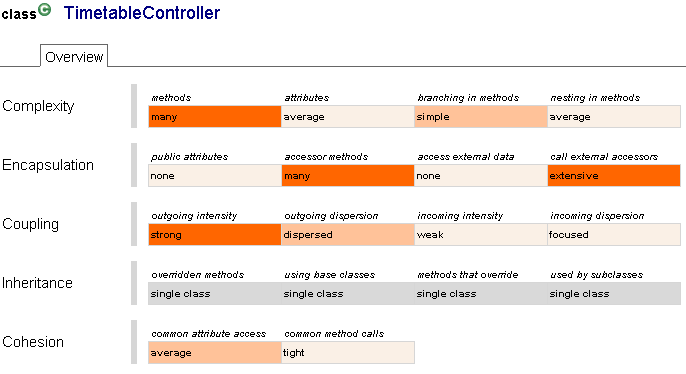
\includegraphics[scale=0.7]{infusion3.PNG}
\caption{Example of Class 'Bad Code Smell' Breakdown using Infusion}
\label{fig:in1}
\end{center}
\end{figure}

An overall quality result is given to the application. Changes can then me made, in order to achieve a benchmark score. It is also worth noting that the use of frameworks, if that decision is made, made have a negative effect on these scores and a cognisance of this is paramount to ensure that time is not spend on corrective action for 'flaws' introduced by design choices. 

\begin{figure}[H]
\begin{center}
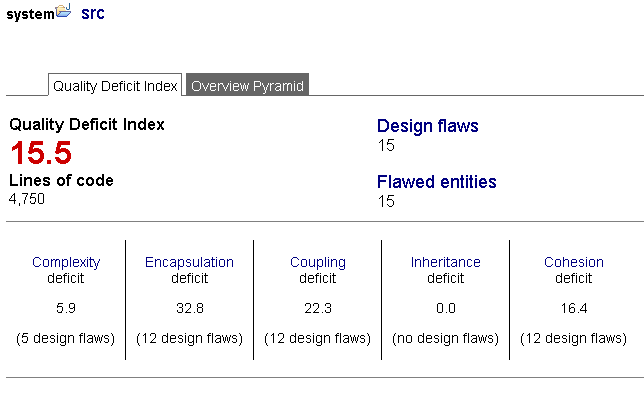
\includegraphics[scale=0.7]{infusion2.PNG}
\caption{Quality Measurement using Infusion}
\end{center}
\end{figure}

\section{Quality Standards}

One standard looked at in this project was \textit{ISO/IEC 25010}. This replaced the old model, \textit{ISO 9126}.

In this model, there is a focus on a number of different attributes. In order to help a project succeed, there attributes must be examined, and acted upon, through the project management process. This is to ensure that the final product is a high quality product, and one that is what the customer wanted. Figure~\ref{fig:iso} shows a summary of the areas that this standard focuses on. 

\begin{enumerate}
\item Functional Stability
\begin{itemize}
\item This refers to the 'appropriateness, accuracy and compliance" of the final product. \parencite{iso}
\end{itemize}

\item Reliability
\begin{itemize}
\item This section focuses on the "availability, fault tolerance and recoverability compliance" of the final product. \parencite{iso}
\end{itemize}

\item Performance Efficiency
\begin{itemize}
\item This is concerned with measurements such as "time behaviour and resource utilisation compliance". \parencite{iso}
\end{itemize}

\item Operability
\begin{itemize}
\item This encompasses usability. and focuses on "ease of use, helpfulness, attractiveness, technical accessibility and learn-ability" of the created system. \parencite{iso}
\end{itemize}

\item Security
\begin{itemize}
\item Within this application, the focus of security is defined by the user requirements. This area will focus on the "confidentiality, integrity, non repudiation, and authenticity" of information within the system.
\end{itemize}

\item Compatibility
\begin{itemize}
\item This area focuses on the effect that different configurations may have on the system. This include "interoperability and replace-ability". \parencite{iso}
\end{itemize}

\item Maintainability
\begin{itemize}
\item This attribute focuses on the design of an application. Key attributes are the "modularity, re-usability, testability and changeability" of the application \parencite{iso}. These attributes normally increase the development time of the application, and thus the risk and cost. 
\end{itemize}

\item Transferability
\begin{itemize}
\item This refers to the "portability and adaptability" of the application to run on different systems, operating systems and configurations. \parencite{iso}
\end{itemize}

\end{enumerate}
\begin{figure}[H]
\caption{Quality Areas Defined by ISO 25010}
\label{fig:iso}
\end{figure}
